% ============================================================
% Q4 – Machine Translation
% ============================================================
\section{Question 4 -- Machine Translation}

\subsection{Dataset: Multi30k (EN$\to$DE)}

Multi30k~\cite{elliott2016multi30k} contains 31\,014 English-German
sentence pairs from image captions (Flickr30k).

\begin{table}[H]
  \centering
  \caption{Multi30k Dataset Splits}
  \label{tab:q4_data}
  \begin{tabular}{lr}
    \toprule
    \textbf{Split} & \textbf{Sentences} \\ \midrule
    Train      & 29{,}000 \\
    Validation & 1{,}014  \\
    Test       & 1{,}000  \\
    \bottomrule
  \end{tabular}
\end{table}

\noindent\textbf{Preprocessing:} Lowercase, punctuation tokenisation (regex),
vocabulary with min-freq=2 (\texttt{<pad>}, \texttt{<unk>}, \texttt{<bos>},
\texttt{<eos>} special tokens), max sequence length 50.

Source vocabulary: 5{,}970\,tokens.
Target vocabulary: 7{,}811\,tokens.

\subsection{Models}

\subsubsection{Model 1 -- Seq2Seq with Bahdanau Attention}

\textbf{Encoder:} 2-layer bidirectional GRU (hidden=256), projects final
states to initialise decoder.
\textbf{Attention:} Bahdanau additive attention aligns each decoder step with
encoder hidden states, computing a context vector as a weighted sum.
\textbf{Decoder:} 2-layer GRU with attention context concatenated to the
embedding; final projection to target vocabulary.
Trained with Adam ($\text{lr}=10^{-3}$), label smoothing=0.1, teacher
forcing=0.5, 15 epochs, batch=128.

\subsubsection{Model 2 -- MarianMT (Helsinki-NLP/opus-mt-en-de)}

\texttt{Helsinki-NLP/opus-mt-en-de}~\cite{tiedemann2020opus} is a
Marian NMT transformer~\cite{vaswani2017attention} (6-layer encoder-decoder)
pre-trained on OPUS multilingual data ($\sim$60\,M parallel sentence pairs).
Used in inference mode with beam search ($k=4$).

\subsection{Results}

\begin{table}[H]
  \centering
  \caption{Machine Translation Results on Multi30k Test Set (EN$\to$DE)}
  \label{tab:q4_results}
  \begin{tabular}{lcccc}
    \toprule
    \textbf{Model} & \textbf{BLEU} & \textbf{ChrF} & \textbf{METEOR} & \textbf{BERTScore} \\
    \midrule
    Seq2Seq + Attn & 0.00   & 0.34  & 0.0484 & -- \\
    MarianMT       & 36.24  & 64.25 & 0.6668 & -- \\
    \bottomrule
  \end{tabular}
\end{table}

\begin{figure}[H]
  \centering
  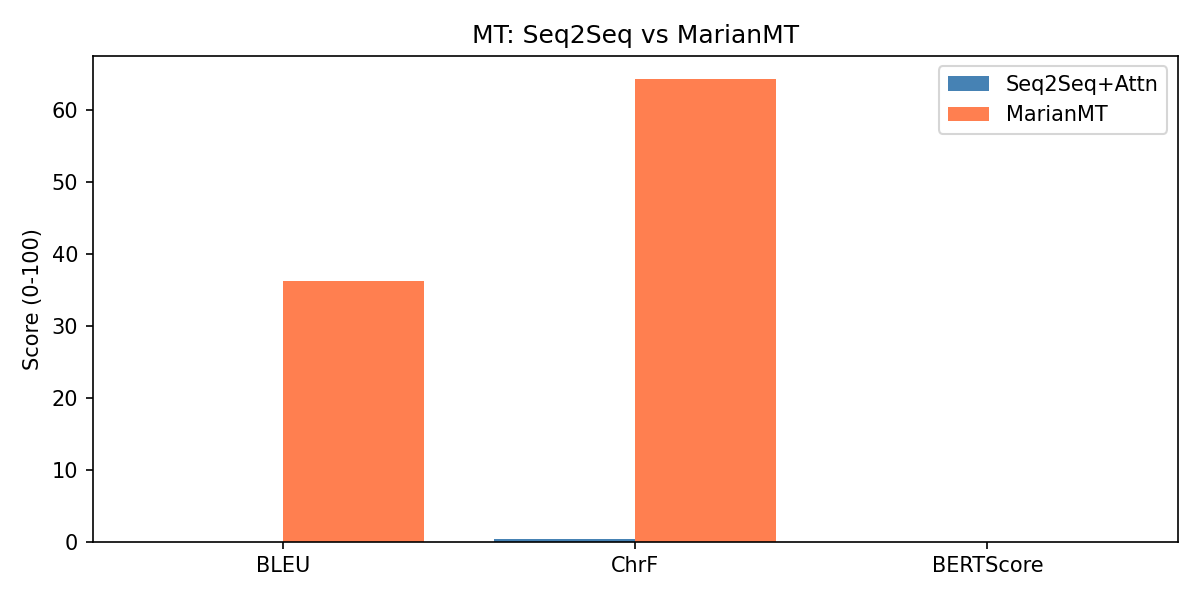
\includegraphics[width=0.75\textwidth]{figures/mt_comparison.png}
  \caption{Machine translation metric comparison: Seq2Seq+Attention vs MarianMT on the Multi30k test set (BLEU, ChrF, METEOR shown; BERTScore could not be computed).}
  \label{fig:mt_comparison}
\end{figure}

\subsection{Qualitative Example}

\begin{table}[H]
  \centering
  \small
  \caption{Translation Example}
  \label{tab:q4_example}
  \begin{tabularx}{\textwidth}{lX}
    \toprule
    \textbf{Source (EN)} & Two men on opposing teams are playing soccer in a field. \\
    \textbf{Reference (DE)} & Zwei M\"anner aus gegnerischen Mannschaften spielen Fu{\ss}ball auf einem Fu{\ss}ballplatz. \\
    \textbf{Seq2Seq + Attn} & \textit{. ,} (model failed to learn translation) \\
    \textbf{MarianMT} & Zwei M\"anner in gegnerischen Teams spielen Fu{\ss}ball auf einem Feld. \\
    \bottomrule
  \end{tabularx}
\end{table}

The Seq2Seq model trained from scratch on only 29\,K sentence pairs (15 epochs)
failed to learn meaningful translations, producing degenerate outputs (e.g.\ ``\textit{. ,}'').
Final perplexity remained high ($\approx$437), indicating the model did not converge.
MarianMT, pre-trained on $\sim$60\,M parallel sentences, produces fluent and accurate
German translations, confirming the decisive advantage of transfer learning for low-resource
sequence-to-sequence tasks.

\subsection{Discussion}

\begin{table}[H]
  \centering
  \caption{Metric Analysis and Architecture Trade-offs}
  \label{tab:q4_discussion}
  \begin{tabular}{lp{5cm}p{5cm}}
    \toprule
    \textbf{Metric} & \textbf{Strength} & \textbf{Limitation} \\
    \midrule
    BLEU    & Standard, fast      & Ignores synonyms; brevity penalty harsh \\
    METEOR  & Synonym + stemming  & Language-resource dependent \\
    ChrF    & Character-level, robust for German compounds & Less intuitive scale \\
    BERTScore & Semantic similarity & Computationally heavy; model-dependent \\
    \bottomrule
  \end{tabular}
\end{table}

The large gap between Seq2Seq and MarianMT across all metrics is attributable
primarily to training data size (29\,K vs $\sim$60\,M parallel sentences).
BLEU and ChrF both reflect near-zero quality for the Seq2Seq model, consistent
with its degenerate outputs. BERTScore could not be computed in this run due to
model compatibility issues with the German target language, but the remaining
three metrics collectively confirm MarianMT's decisive superiority.
